\documentclass{beamer}
\usepackage{amsmath}
\usepackage{mathtools}
\usepackage[outline]{contour}

\mode<presentation>
{
  \useoutertheme{default}
}

\beamertemplatenavigationsymbolsempty
\setbeamertemplate{frametitle}[default][center]
%\setbeamercolor{frametitle}{fg=white}
%\setbeamercolor{background canvas}{bg=black}
%\setbeamercolor{normal text}{fg=white}
%\usepackage[dvipsnames]{xcolor}
\definecolor{cyan}{rgb}{0,1,1}
\definecolor{yellow}{rgb}{1,1,0}
\definecolor{magenta}{rgb}{1,0,1}

\title{Numerical methods for multi-stage models of cancer incidence}
\author{Chay Paterson}
\institute{University of Manchester}
\date{\today}

\begin{document}

\frame{\titlepage}

\begin{frame}
    \frametitle{Multi-stage models}
    \framesubtitle{P. Armitage and R. Doll\footnotemark[12]}

    \begin{columns}
        \begin{column}{0.5\textwidth}
        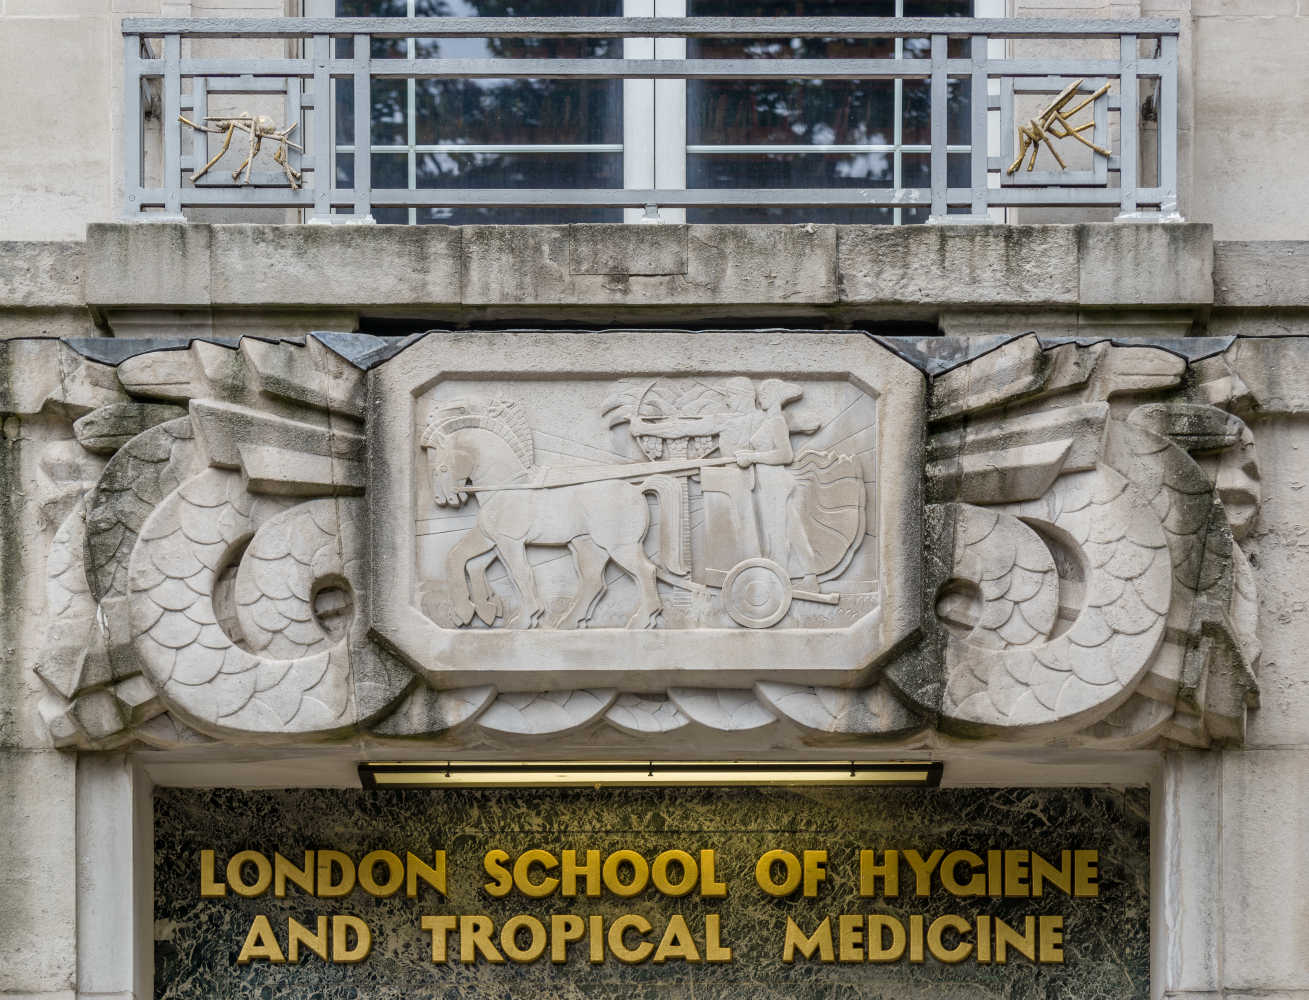
\includegraphics[width=\textwidth]{figures/LSHTM-small.jpg}
        \end{column}
        \begin{column}{0.5\textwidth}
        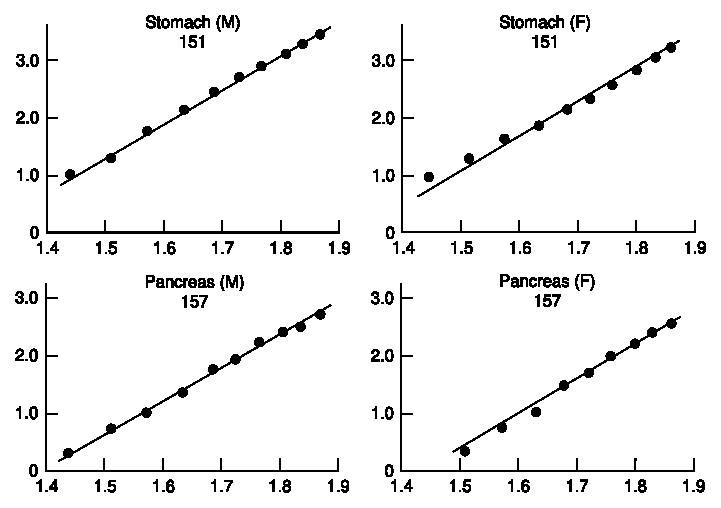
\includegraphics[width=\textwidth]{figures/PArmitageRDoll_1954_6602297.pdf}
        \end{column}
    \end{columns}


\footnotetext[1]{P. Armitage and R. Doll, British Journal of Cancer 1954; 8: 1–12}
\footnotetext[2]{P. Armitage and R. Doll, British Journal of Cancer 1957; 11(2): 161-169}
\end{frame}

\begin{frame}
    \frametitle{Multi-stage models}
    \framesubtitle{A.G. Knudson\footnotemark[12]}

    \begin{columns}
        \begin{column}{0.5\textwidth}
            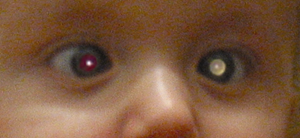
\includegraphics[width=0.90\textwidth]{figures/Rb_whiteeye.PNG}
            \;
            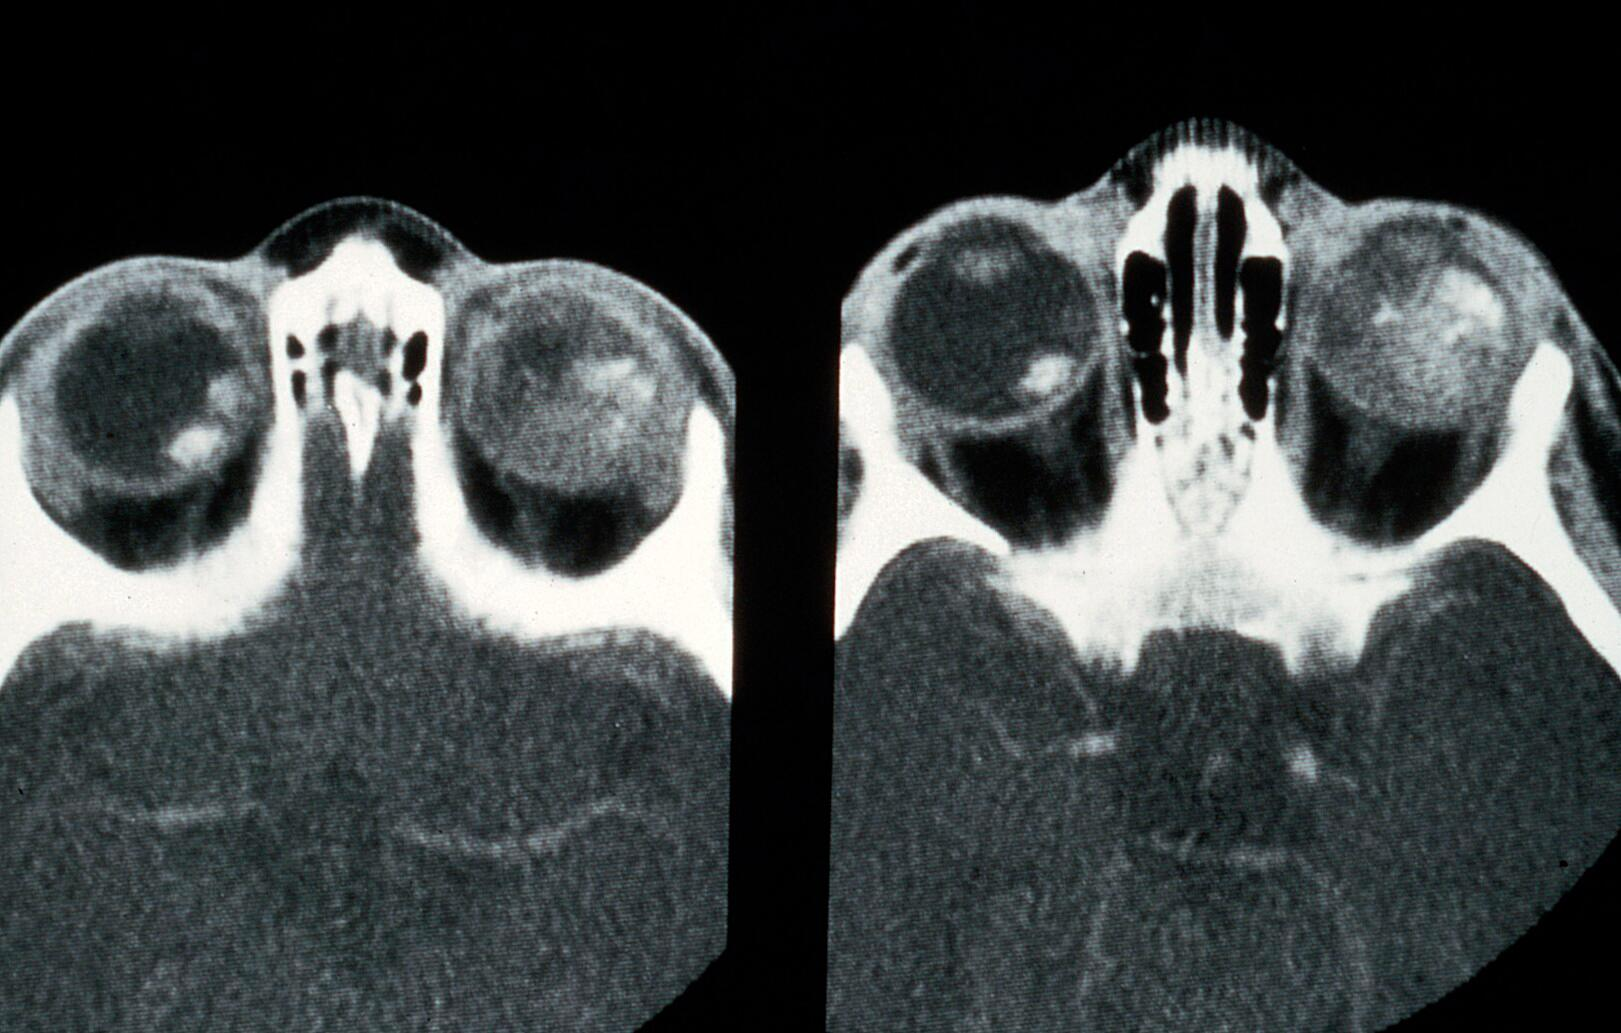
\includegraphics[width=0.90\textwidth]{figures/retinoblastoma.jpg}
        \end{column}
        \begin{column}{0.5\textwidth}
            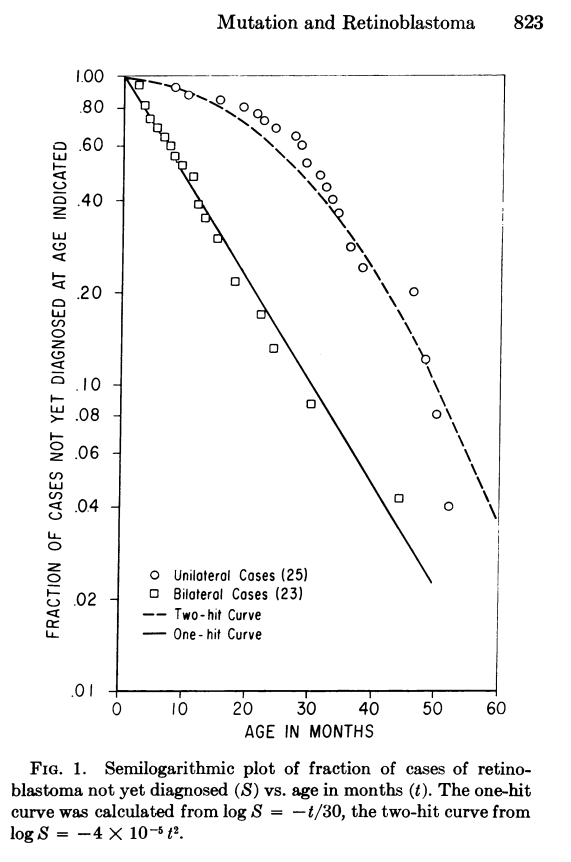
\includegraphics[width=0.90\textwidth]{figures/Screenshot_2022-10-31_11-57-01.png}
        \end{column}
    \end{columns}

\footnotetext[1]{AG. Knudson, PNAS 68.4 (1971): 820-823.}
\footnotetext[2]{F. Michor, Y. Iwasa and MA. Nowak, Nature Reviews Cancer 2004; 4: 197-205 doi:10.1038/nrc1295}
\end{frame}


\begin{frame}
    \frametitle{How do these studies work?}

    What are the relevant observables in this type of longitudinal study \& data
    analysis? 

    Follow a cohort that contains some of our patients in the study:

    \begin{itemize}
        \item Age-specific incidence $I(a)$: number of new cases are
        recorded in the cohort with ages between $a$ and $a + da$
        \item Hazard function $h(a)$: \emph{rate} with which individuals in
        cohort at age $a$ are diagnosed.
        \item Survival function $S(a)$: proportion of individuals in cohort who
        have not yet been diagnosed by age $a$
    \end{itemize}
\end{frame}

\begin{frame}
    \frametitle{How do these studies work?}
    \framesubtitle{How are these variables related?}

    Denote by $n(a)$ the number of people in the reference cohort that remain
    undiagnosed by age $a$. Then:

    \begin{equation}
        I(a) = n(a) h(a) da
    \end{equation}
    and $n(a)$ is actually determined by $S(a)$ and the initial reference
    population of the cohort (num. of babies born at same time) $n(0)$:

    \begin{equation}
        n(a) = n(0) S(a)
    \end{equation}
    so, logically:

    \begin{equation}
        I(a) = n(0) S(a) h(a) da
    \end{equation}
\end{frame}

\begin{frame}
    \frametitle{How do these studies work?}
    \framesubtitle{How are these variables related?}

    But it's also true that the number of people diagnosed during the period 
    $[a, a + da)$ must be:

    \begin{equation}
        n(a) - n(a + da) = I(a)
    \end{equation}
    hence:

    \begin{equation*}
        I(a) = n(a) - n(a + da) = n(0) (S(a) - S(a + da))
    \end{equation*}

    \begin{equation*}
    \implies S(a) - S(a + da) = S(a) h(a) da
    \end{equation*}

    \begin{equation*}
    \implies h(a) = (S(a) - S(a + da)) / (S(a) da) \rightarrow -\frac{d \ln S}{ da}
    \end{equation*}
    as $da \rightarrow 0$.

\end{frame}

\begin{frame}
    \frametitle{So what?}

    \begin{itemize}
        \item The survival curve S(a) determines everything else of interest.
        \item The model determines the survival curve. The parameters determine
        the model. We want to know what model+parameters best agree with
        data from studies.
        \item To fit (or ``train'') the model to longitudinal data, we need to compute $S(a)$!
    \end{itemize}

    \;

    This is the central mathematical problem in cancer epidemiology. \emph{How do we compute $S$?}
\end{frame}

\begin{frame}
    \frametitle{Multi-stage clonal expansion models}
    \framesubtitle{2-3 rate limiting steps\footnotemark[123]}
    % TODO present both models
    % ie include Armitage Doll 1957 model, cite Jo Ivasa
    Problem: how to compute $S(t)$ for a given model?

    \begin{columns}
        \begin{column}{0.5\textwidth}
        \begin{center}
        % multi-stage clonal expansion
        \end{center}
        Different methods:
        Fast:
        \begin{itemize}
            \item Armitage + Doll's approximation\footnotemark[1]
            \item Moolgavkar + Venzon's quadrature\footnotemark[2]
        \end{itemize}
        Very slow:
        \begin{itemize}
            \item Gillespie algorithm + sampling \footnotemark[3]
        \end{itemize}
        \end{column}
        \begin{column}{0.5\textwidth}
        \begin{center}
            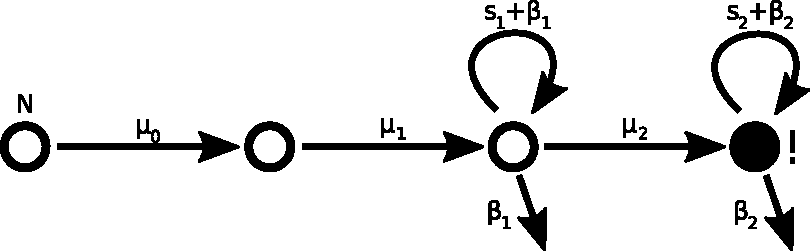
\includegraphics[width=1.00\textwidth]{figures/diagram3}
            $\downarrow?$
            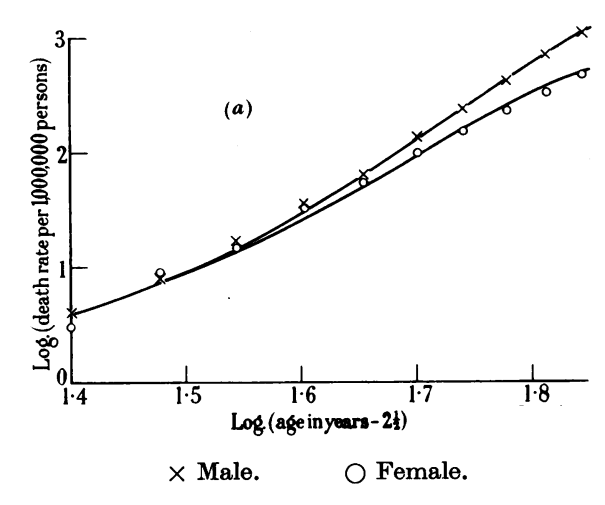
\includegraphics[width=0.75\textwidth]{figures/ArmitageDoll1957_4A.png}
        \end{center}
        \end{column}
    \end{columns}

    % TODO add figure from Armitage Doll 1957 etc.
\footnotetext[1]{P. Armitage and R. Doll, British Journal of Cancer 1957; 11(2): 161-169}
\footnotetext[2]{S. Moolgavkar and G. Luebeck, JNCI 1992; 84(8): 610-618}
\footnotetext[3]{C. Paterson, I. Bozic, H. Clevers, PNAS 2020; 117(34): 20681-20688 (supp. material)}
\end{frame}


\begin{frame}
    \frametitle{Armitage and Doll's approximation}

    \begin{columns}
        \begin{column}{0.5\textwidth}
            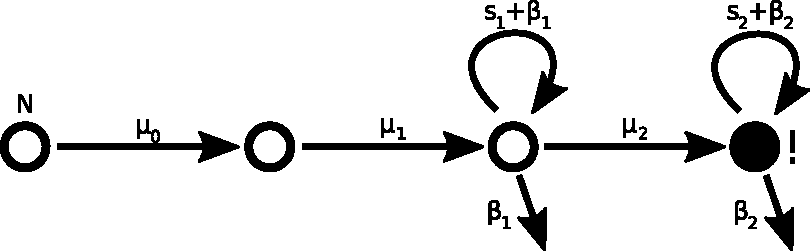
\includegraphics[width=1.00\textwidth]{figures/diagram3}
            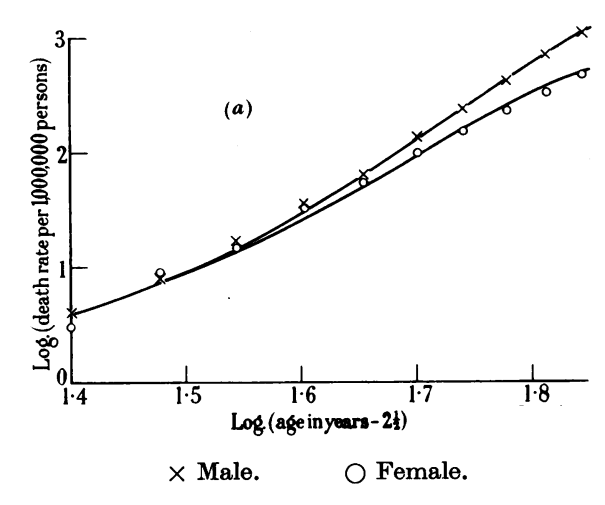
\includegraphics[width=0.75\textwidth]{figures/ArmitageDoll1957_4A.png}
        \end{column}
        \begin{column}{0.5\textwidth}
        \begin{itemize}
            \item Assume all the probabilities are small
            \item Then the relevant probability $S(a)$ is expressible in terms
            of expected values/population means, which implies
        \end{itemize}
        \begin{equation}
            S(a) \propto a^k (e^{s a} - 1)
        \end{equation}
        with constants $k$ and $s$.
        \begin{itemize}
            \item Don't use correlations, variances, or higher moments in stem
            cell populations -- just ignore these.
        \end{itemize}
        \end{column}
    \end{columns}
\end{frame}

\begin{frame}
    \frametitle{Armitage and Doll's approximation}

    What's wrong with this?
    \begin{itemize}
        \item In old age, the approximation will fail -- it assumes the probabilities
        are small, we cannot use it when we know the probabilities will be high.
        \item Predicts that cancer risk should increase in an accelerating way with age
        \item (Which it doesn't -- the hazard $h(a)$ levels off (R. Meza))
    \end{itemize}

    Which leads us to...
\end{frame}


\begin{frame}
    \frametitle{The ``gold standard'': Moolgavkar, Venzon, and Luebeck's approach}

    \begin{columns}
        \begin{column}{0.5\textwidth}
            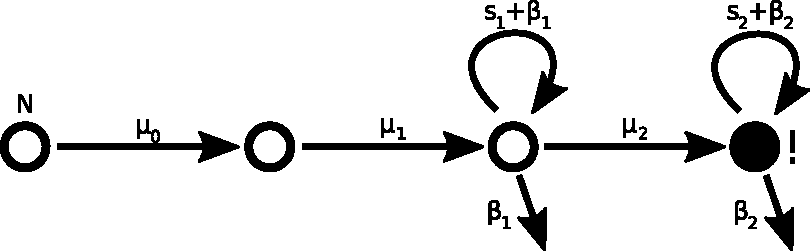
\includegraphics[width=1.00\textwidth]{figures/diagram3}
            Same basic model as Armitage and Doll, but solved exactly (no
            approximations).
        \end{column}
        \begin{column}{0.5\textwidth}
        \begin{itemize}
            \item Don't assume anything about probabilities or correlations.
            \item Transform the equations, and try to solve for the distribution directly.
        \end{itemize}
        \end{column}
    \end{columns}
\end{frame}

\begin{frame}
    \frametitle{Moolgavkar, Venzon, and Luebeck's approach}
    \framesubtitle{How it works}
    Define a set of generating functions $Psi_k$ (one for each stem cell
    population $k$):

    \begin{equation}
        \Psi_k(t,\vec{x}) := \mathbb{E}\left[\prod_j x_j^{N_j}|N_k = 1, N_{j\neq k} = 0\right]
    \end{equation}

    Derive Kolmogorov backward equation to evolve this backwards in time:

    \begin{equation}
        \frac{d \Psi_k}{dt} = (... \Psi_k \; and \; \Psi_{k+1} ...)
    \end{equation}
    and we can compute the survival curve $S(a)$ from

    \begin{equation}
        S(a) = \Psi_0(a, 1, 1, 1, ..., 1, 0)
    \end{equation}
\end{frame}

\begin{frame}
    \frametitle{Moolgavkar, Venzon, and Luebeck's approach}
    \framesubtitle{How it works}
    In fact, we get a recursive hierarchy of $S$ curves for different models:

    \begin{equation}
        S_k(a) = \exp\left(... \int_{z=0}^a S_{k+1}(z) ... dz\right)
    \end{equation}

    which can be evaluated very efficiently with numerical integration. This has
    been the best available method for evaluating $S(a)$ in multi-stage models
    since about 1992. (See: Bhat, Georg's package on R-CRAN).
    
    \;

    So what's the problem with the ``classical'' approach?
\end{frame}

\begin{frame}
    \frametitle{Models on graphs}
    \begin{columns}
        \begin{column}{0.5\textwidth}
        \begin{enumerate}
            \item The classical approach is specialised for 2- and 3-hit models:
            it doesn't work on graphs
            \item To study \textbf{specific genes} and mechanisms of interest
            (SNVs, LOH, CNA, etc.), we need to evaluate $S(a)$ for a model
            defined on a graph (right)
            \item What methods do we actually have?
        \end{enumerate}
        \end{column}
        \begin{column}{0.5\textwidth}
        \begin{center}
            \small{example model}
        \end{center}
            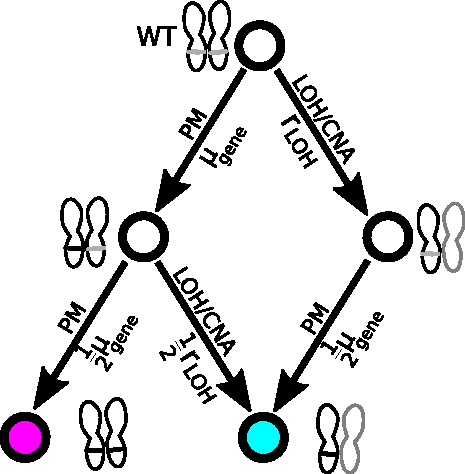
\includegraphics[width=\textwidth]{figures/diagram4}
        \end{column}
    \end{columns}

    \;

    \begin{center}
        This gets us the incidence of \emph{specific karyotypes}
    \end{center}
\end{frame}


\begin{frame}
    \frametitle{Colorectal adenocarcinoma model}
    \begin{columns}
        \begin{column}{0.5\textwidth}
        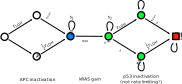
\includegraphics[width=1.0\textwidth]{figures/diagram7}
        \begin{itemize}
            \item Can use A-D type approximation, or stochastic simulations
            %\item Conditional path probabilities $P(X_i)$ encode fitnesses
        \end{itemize}
        but:
        \begin{itemize}
            \item Mean-field breaks down at old ages / large probabilities
            \item Stochastic simulations are \emph{extremely slow}
        \end{itemize}
        \end{column}
        \begin{column}{0.5\textwidth}
        % graph from our PNAS paper
        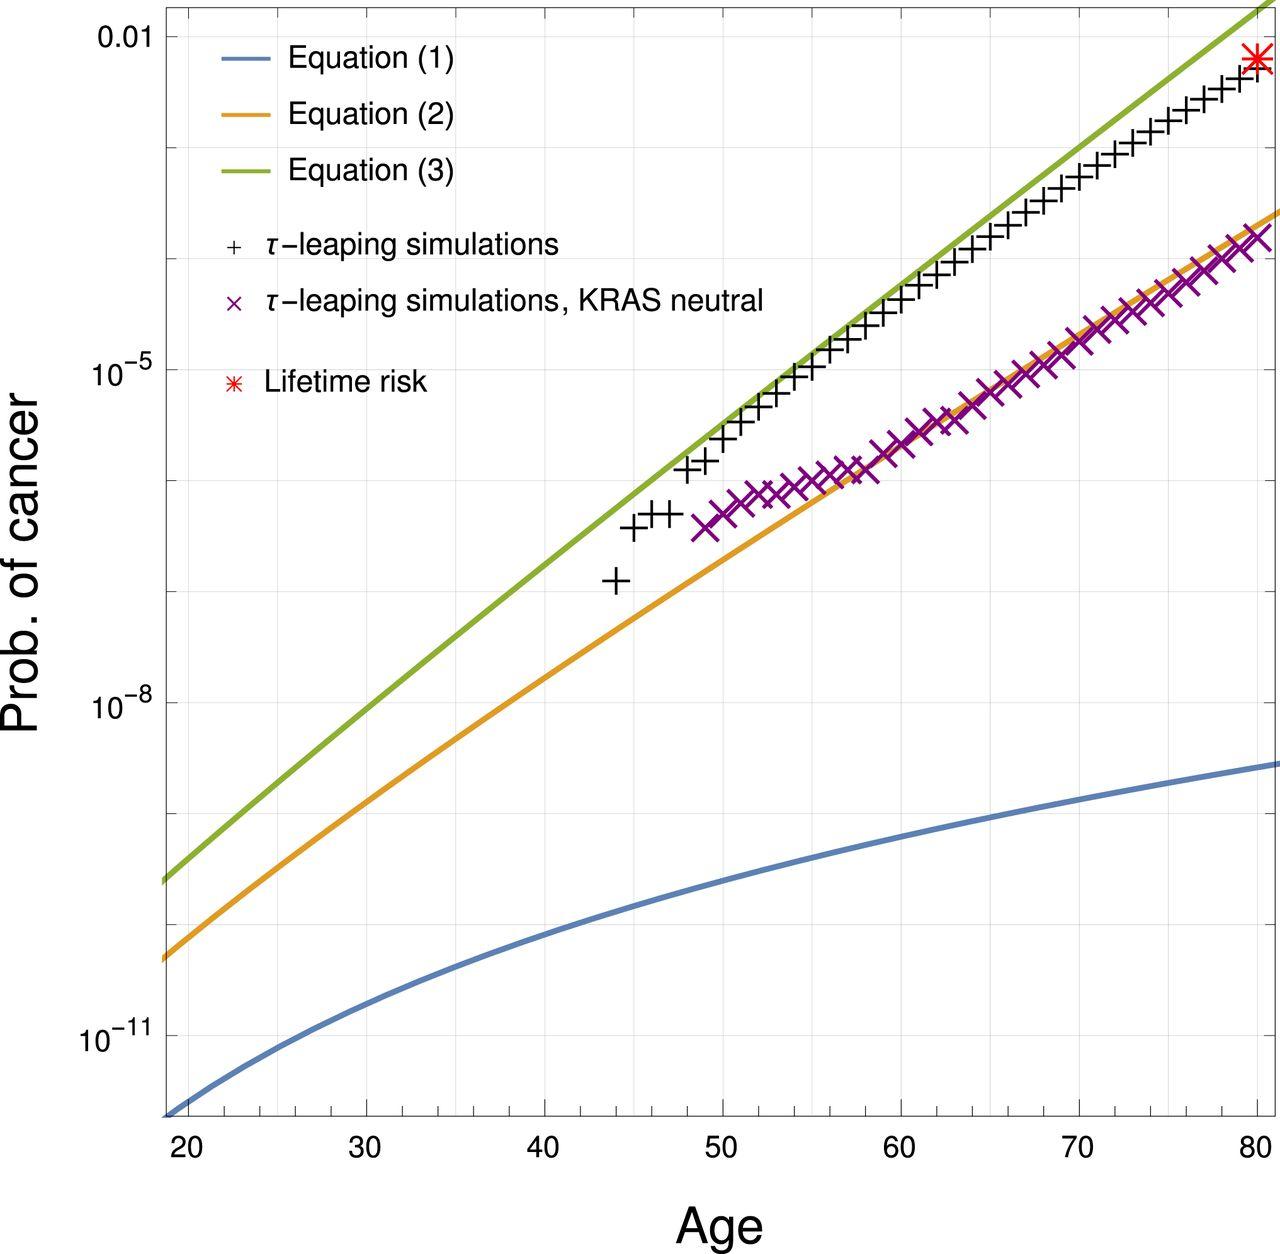
\includegraphics[width=\textwidth]{figures/F2.large.jpg}
        \end{column}
    \end{columns}

\footnotetext[1]{C. Paterson, I. Bozic, H. Clevers, PNAS 2020; 117(34): 20681-20688}
\end{frame}

\begin{frame}
    \frametitle{New idea!}
    Define a more general generating function $\Psi$:

    \begin{equation}
        \Psi(t, \vec{q}) = \mathbb{E}[\left[\prod_j q_j^{N_j}\right]
    \end{equation}

    and derive Kolmogorov FORWARD equations instead. Then we can numerically
    integrate these, and get survival curves $S_i(a)$ for different types of
    cancer $i$. E.G. tumours with clonal LOH, or no clonal LOH.

    \begin{equation}
        S_i = \Psi(t, q_j =1, \dots, q_i = 0)
    \end{equation}
    People knew about this approach for a long time (since 1988ish) but it was never
    considered as useful as backward equations.

\footnotetext[1]{e.g. DW Quinn, S Moolgavkar both described the basic version at about this time}
\end{frame}

\begin{frame}
    \frametitle{Easier said than done}

    In and out, twenty minute adventure...

    \;

    \vphantom{Five years later...}
\end{frame}

\begin{frame}
    \frametitle{Easier said than done}

    In and out, twenty minute adventure...

    \;

    {Five years later...}
\end{frame}

\begin{frame}
    \frametitle{Fast forward method}

    \begin{columns}
        \begin{column}{0.5\textwidth}
    Using the big generating function $\Psi$, find the Kolmogorov forward
    equations:

    \begin{equation}
        \frac{d \Psi}{ dt} = \vec{X} \cdot \nabla \Psi
    \end{equation}

    This can be solved using the method of characteristics, so we can instead
    integrate

    \begin{equation}
        \frac{d \vec{\gamma}}{ dt} = \vec{X}
    \end{equation}
    numerically, using a method like improved Euler integration.


        \end{column}
        \begin{column}{0.5\textwidth}
            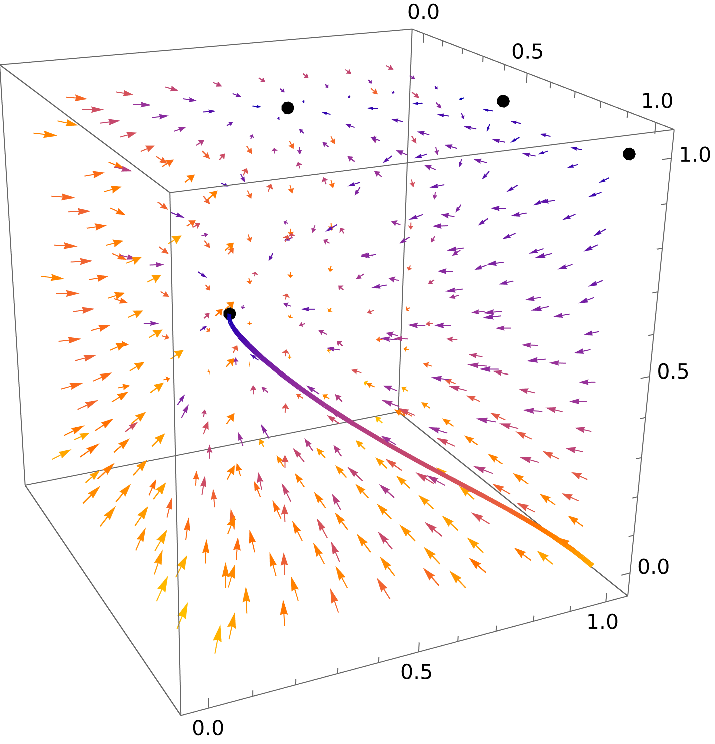
\includegraphics[width=\textwidth]{figures/flowcube1}

            \;

            The vector field $\vec{X}$ and a characteristic $\vec{\gamma}$
        \end{column}
    \end{columns}
\end{frame}

\begin{frame}
    \frametitle{Fast forward method}

    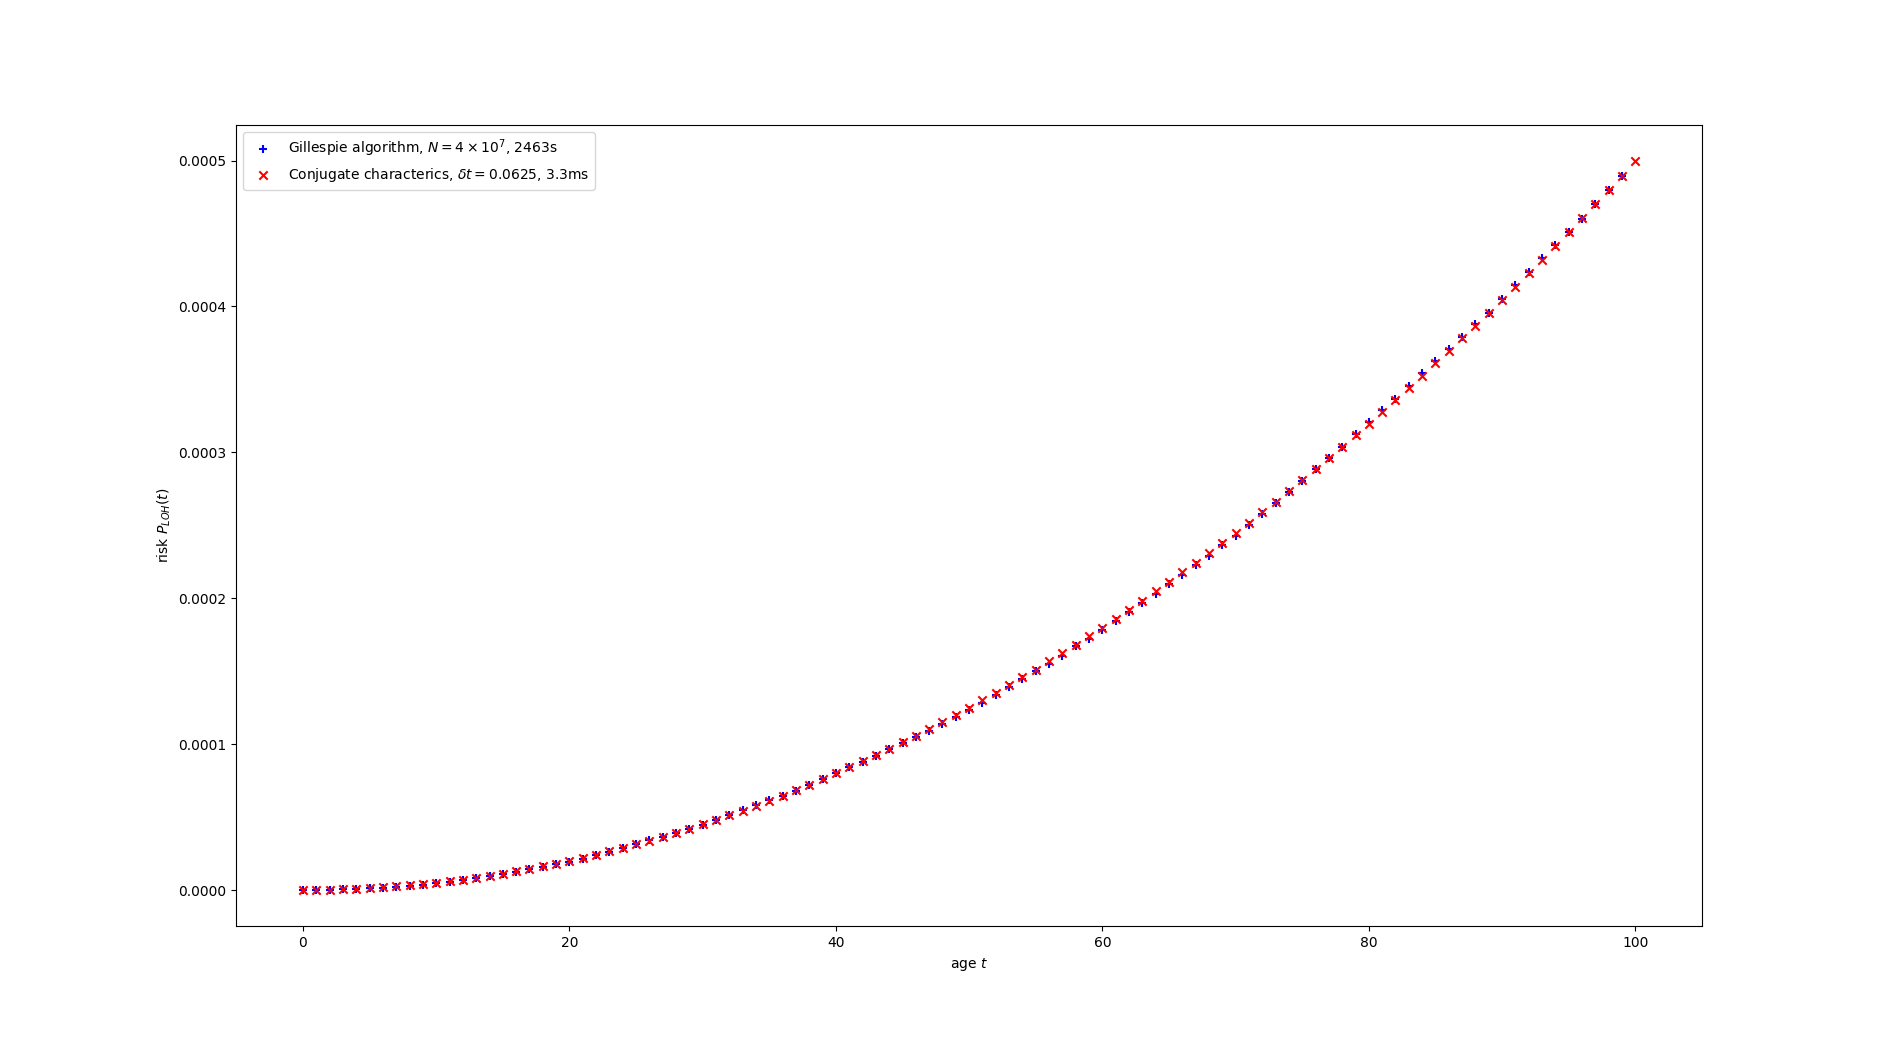
\includegraphics[width=\textwidth]{figures/Figure_1.png}


    Gillespie algorithm vs fast forward method:

    Gillespie: 2500s

    Fast forward: 3ms (~1ms for same error)
\end{frame}


\begin{frame}

    To compare the two methods, ask under what conditions the errors are
    comparable. Stochastic algorithms have 

    \begin{equation}
        \epsilon \sim N^{-1/2}
    \end{equation}
    and will thus need
    
    \begin{equation}
        N \sim \mathcal{O}(\epsilon^{-2})
    \end{equation}
    runs, and overall runtime $T \propto N$.

\end{frame}

\begin{frame}
    \frametitle{Fast forward method}
    \framesubtitle{Error analysis}
    Fast forward method has

    \begin{equation}
        \epsilon \sim \Delta t^2
    \end{equation}
    and runs in 
    \begin{equation}
        T \sim \Delta t^{-1} \sim \mathcal{O}(\epsilon^{-1/2})
    \end{equation}
    so new runtime $\sim \mathcal{O}\left(\right.$ old runtime
    $\left.^{1/4}\right)$.

    \;

    Amazing!
\end{frame}

\begin{frame}
    \frametitle{Fast forward method}
    \framesubtitle{Error analysis}
    \begin{center}
        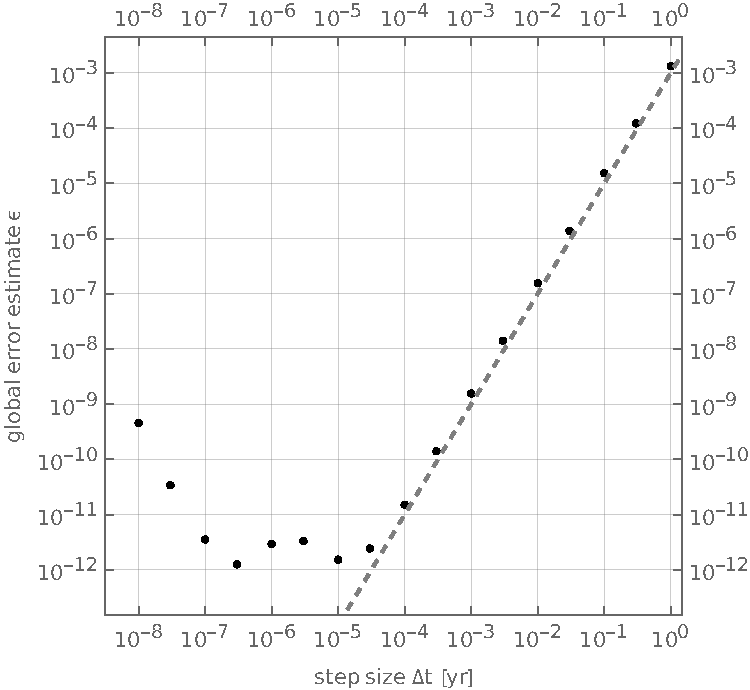
\includegraphics[height=0.9\textheight]{figures/errors2}
    \end{center}
\end{frame}

\begin{frame}
    \frametitle{Fast forward method}
    \framesubtitle{Error analysis}

    Why wasn't this used before? DW Quinn and S Moolgavkar both studied forward
    equation+characteristic methods, but used Euler integration, which has
    \begin{equation}
        \epsilon \sim \Delta t
    \end{equation}
    and required two passes, so it ran in
    \begin{equation}
        T \sim \Delta t^{-2} \sim \mathcal{O}(\epsilon^{-2})
    \end{equation}
    this is asymptotically just as bad as random sampling! You only get a
    constant speed-up.
\end{frame}


\begin{frame}
    \frametitle{Fast forward method}
    \framesubtitle{Parameter inference}

    \begin{columns}
        \begin{column}{0.5\textwidth}
        \begin{itemize}
            \item Can use fast forward method to quickly compute likelihoods
            \item Can then test different parameters in e.g. simulated annealing, and maximise the likelihood!
            \item This process can run in about a minute -- this would be impossible with
        Gillespie's algorithm and e.g. ABC.
        \end{itemize}
        \end{column}
        \begin{column}{0.5\textwidth}
            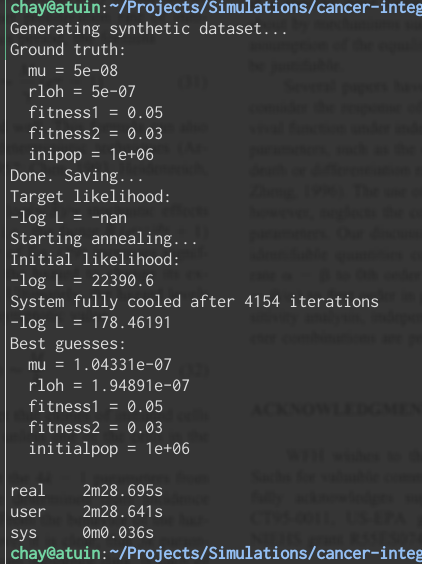
\includegraphics[width=1.0\textwidth]{figures/maxlikelihood.png}
        \end{column}
    \end{columns}
\end{frame}

\begin{frame}
    \frametitle{Fast forward method}
    \framesubtitle{Parameter inference}

Gets the right order of magnitude for some parameters, but:

\begin{itemize}
    \item Very sensitive to choice of neighbours.
    \item Very sensitive to cooling schedule. 
    \item Some parameters (initial stem cell population $N_0$) are not identifiable.
    This is a universal problem though.
\end{itemize}

Still a work in progress... But a great result!
\end{frame}

\end{document}
